\documentclass[tikz,border=2pt]{standalone}
\usepackage{amsmath}
\usetikzlibrary{arrows.meta}
\begin{document}
% rep(1:3, ...): times = 2 -> 1 2 3 1 2 3; each = 2 -> 1 1 2 2 3 3;
% times = 1:3 -> 1 2 2 3 3 3; length.out = 5 -> 1 2 3 1 2 (last copy cut).
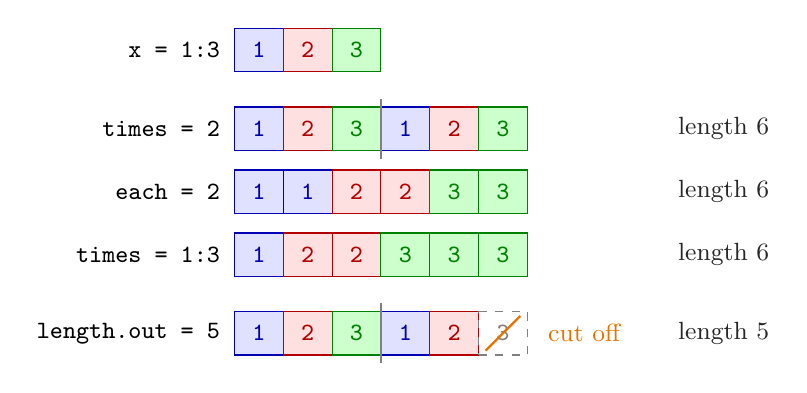
\begin{tikzpicture}[font=\small, >={Latex[length=2mm]},
  cell/.style={draw, minimum width=0.62cm, minimum height=0.55cm, inner sep=1pt, font=\small\ttfamily},
  v1/.style={cell, draw=blue!70!black, fill=blue!12, text=blue!70!black},
  v2/.style={cell, draw=red!70!black, fill=red!12, text=red!70!black},
  v3/.style={cell, draw=green!50!black, fill=green!20, text=green!50!black},
  cut/.style={cell, draw=gray, dashed, text=gray},
  lab/.style={anchor=east, font=\small\ttfamily}]
  \def\w{0.62}
  \node[lab] at (0.25,0) {x = 1:3};
  \foreach \v [count=\i] in {1,2,3} { \node[v\v] at (\w*\i,0) {\v}; }
  \node[lab] at (0.25,-1.0) {times = 2};
  \foreach \v [count=\i] in {1,2,3,1,2,3} { \node[v\v] at (\w*\i,-1.0) {\v}; }
  \draw[gray, thick] (\w*3.5,-0.62) -- (\w*3.5,-1.38);
  \node[lab] at (0.25,-1.8) {each = 2};
  \foreach \v [count=\i] in {1,1,2,2,3,3} { \node[v\v] at (\w*\i,-1.8) {\v}; }
  \node[lab] at (0.25,-2.6) {times = 1:3};
  \foreach \v [count=\i] in {1,2,2,3,3,3} { \node[v\v] at (\w*\i,-2.6) {\v}; }
  \node[lab] at (0.25,-3.6) {length.out = 5};
  \foreach \v [count=\i] in {1,2,3,1,2} { \node[v\v] at (\w*\i,-3.6) {\v}; }
  \draw[gray, thick] (\w*3.5,-3.22) -- (\w*3.5,-3.98);
  \node[cut] at (\w*6,-3.6) {3};
  \draw[orange!90!black, thick] (\w*6-0.22,-3.82) -- (\w*6+0.22,-3.38);
  \node[anchor=west, orange!90!black] at (\w*6+0.45,-3.6) {cut off};
  % lengths on the right
  \foreach \y/\n in {-1.0/6, -1.8/6, -2.6/6, -3.6/5} {
    \node[anchor=west, gray!30!black] at (\w*6+2.1,\y) {length \n};
  }
\end{tikzpicture}
\end{document}
